\chapter{Appendix}\label{chap:appendix}

\subsection{Learning from the inertial EuRoC dataset}\label{sec:euroc_filtering}

The EuRoC dataset \cite{Burri25012016} contains IMU measurements at 200Hz and 6-DoF ground-truth estimates captured using a Vicon motion capture system at 100 Hz. 
After some testing in section \ref{sec:speed_reg}, we empirically show that a heavily parametrized deep model can be successful at fitting the training datasets for partial state prediction from just the IMU data, whether that is an overfit or not.
To be able to do it, however, a low-pass pre-processing of the EuRoC dataset is employed, as the IMU data and especially the accelerometer data are quite noisy for this dataset.
This low pass filtering is found to be \textbf{critical} when fitting in the model, as without it even a model with 18 million parameters is not able to overfit a 1-dimensional output.

The EuRoC flights used (Machine Hall 1 \& 2) can be divided in two sequences separated by a still period.
During the first 20 seconds approximately, the drone is picked up and moved by hand; then it is left back on the floor for a few more seconds, and finally (starting around second 30) it is remotely piloted for a longer period of time.
This fact helps us realize that the increased noise in the accelerometer is present only during the second sequence, when the drone is flying, as it can be seen in Figure \ref{fig:filtEuroc} (top).
We thus hypothesize that the increased noise is probably produced by the vibration of the rotors, and proceed to study if it can be safely removed with some filtering technique.

\subsubsection{Low pass filtering of MAV's inertial data}

After inspection of the Short Time Fourier Transforms (STFT) of the IMU and the ground truth data, we confirm that there is a very significant increase of high frequency components during the second sequence, which are completely not present in the first sequence (especially around the frequency range of 20-30 Hz for the $y$ component).
This leads to the hypothesis that rotor noise can be safely removed with a low-pass filter without affecting to the overall IMU data quality.
The filter employed is chosen to be the Butterworth filter, which has two design parameters: the degree of the filter $n$ and the cutoff frequency $f_0$. 
The reason behind the usage of the Butterworth filter, is that it keeps the frequencies in the pass band almost unaltered, which in our case we assume contain the most relevant information about the trajectory of the flying unit.
We chose $f_0$ to be 10Hz, as in the STFT diagram the components above this frequency in the first part (manual motion) are significantly reduced.
We then select $n$ by trial and error, picking up the smallest value that still \emph{attenuates enough}, the high frequency noise, so that the noisy region resembles the manual motion. 
We find $n=3$ to be a good value for this parameter, which led to the results shown in Figure \ref{fig:accSTFT}.
\begin{figure}
    \centering
    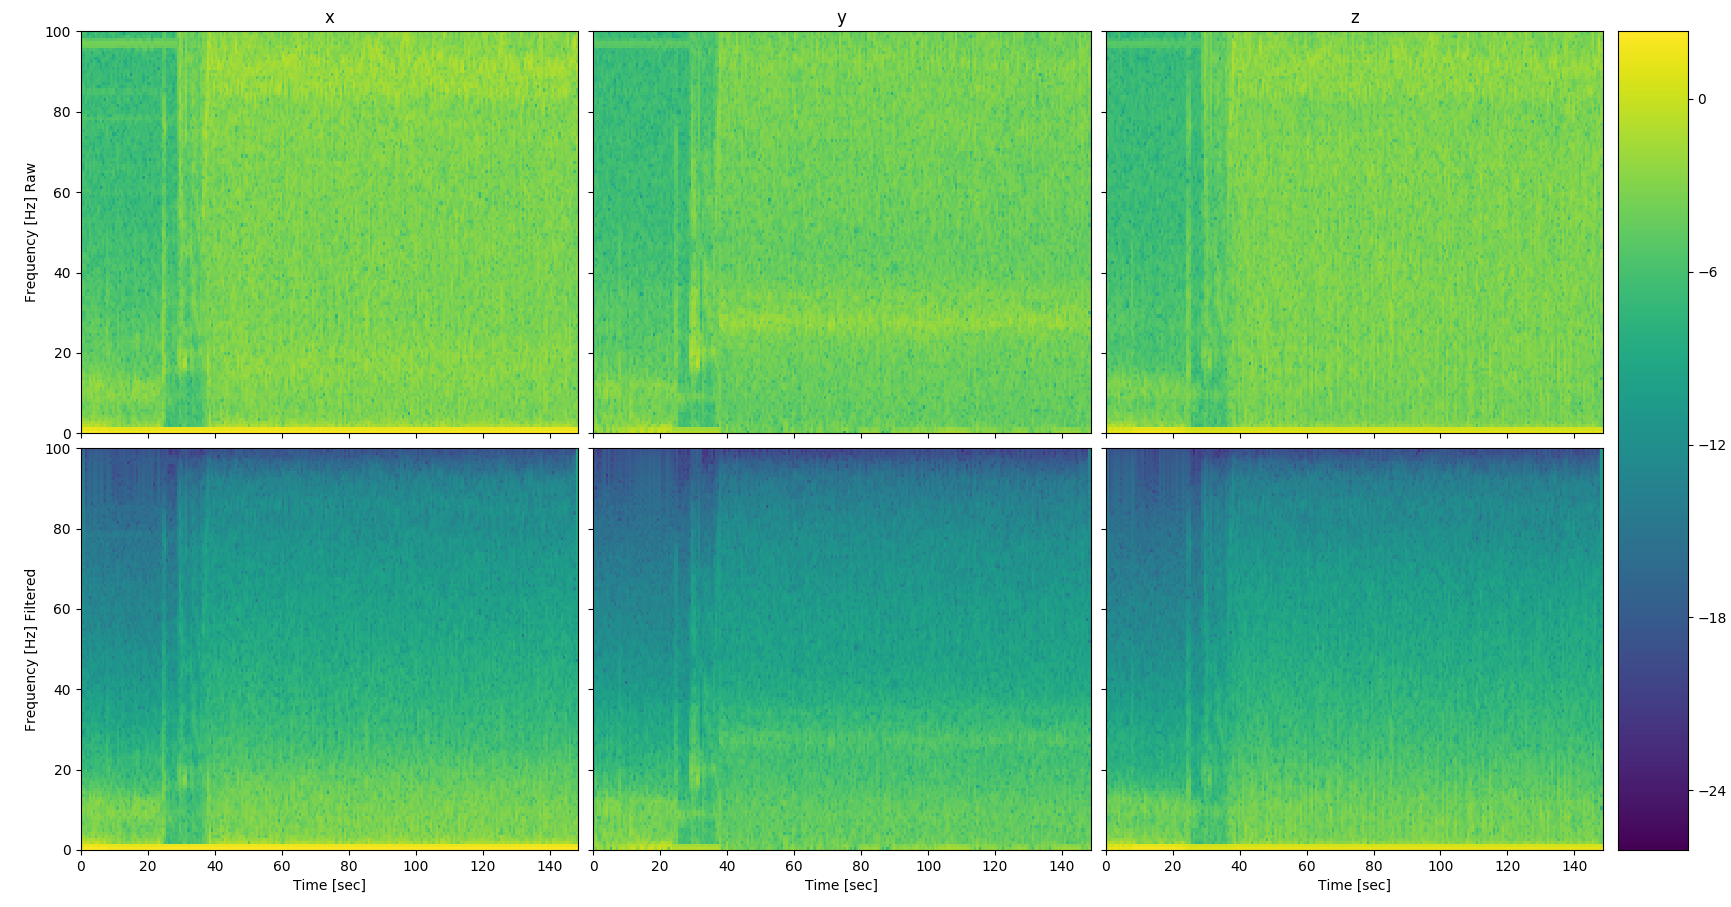
\includegraphics[width=\textwidth,height=\textheight,keepaspectratio]{thesis_template/img/accSTFT.png} 
    \caption{STFT of the accelerometer readings before (top row) and after (bottom row) the application of a low-pass filter (log scale)}
    \label{fig:accSTFT}
\end{figure}
It can also be appreciated in the time domain signal (Figure \ref{fig:filtEuroc} (bottom) that a large portion of the noise has indeed disappeared.
This, more importantly, leads to the model being able to fit with much more precision the training data.
One may also notice in Figure \ref{fig:filtEuroc}, that the \emph{flat} region of the dataset has been expanded. 
We do this because we empirically find that it helped to determine the \emph{resting state} for the model, i.e. when the drone is not moving at all. 
\begin{figure}
    \centering
    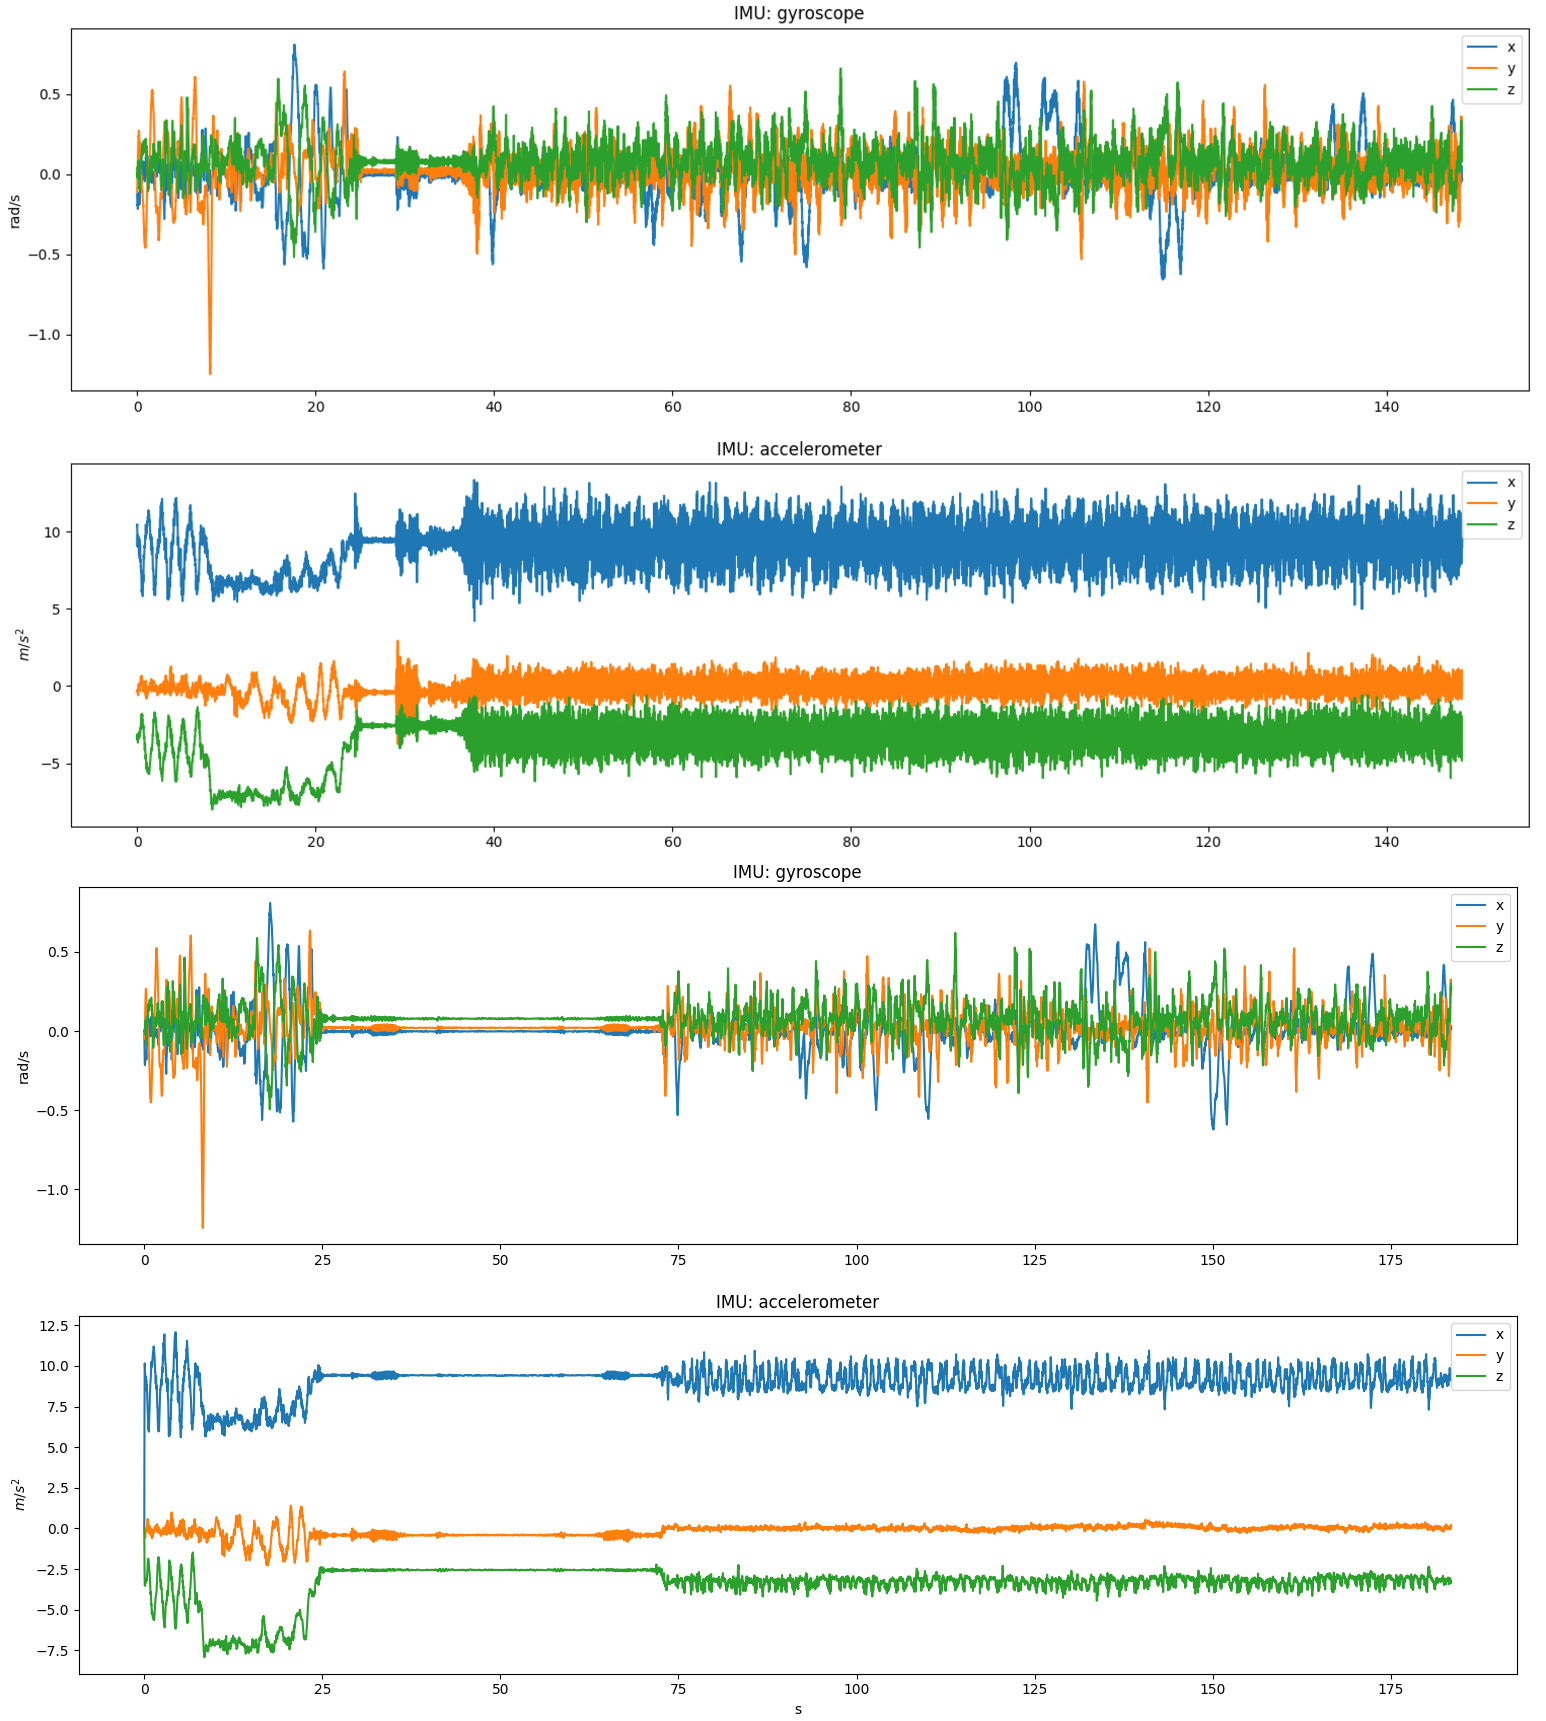
\includegraphics[width=\textwidth,height=\textheight,keepaspectratio]{thesis_template/img/euroc_imu_filtering.jpg} 
    \caption{Unfiltered (top two) and filtered (bottom two) IMU readings of flight "Machine Hall 2" from the Euroc dataset}
    \label{fig:filtEuroc}
\end{figure}

As a last verification step, in Section \ref{sec:speed_regression_model}, we evaluate the performance of the model with the ideal version of the EuRoC dataset with and without noise, and check that its predictions are nearly identical.

For this reason, from we always perform this low-pass filtering for all our inertial data, as it was found to help a lot during training.

\cleardoublepage